% \special{dvipdfmx:config z 0} % disable pdf compress to boost compilation time, comment this out for release
\documentclass{article}

\usepackage{amsmath, amsfonts, amsthm, amssymb} 
\usepackage{listings}
\usepackage{graphicx}
\usepackage{float}
\usepackage{subfigure}
\usepackage{geometry}
\usepackage{hyperref}
\usepackage[parfill]{parskip} % no newline indent
\usepackage{enumitem} % enumerate / ordered list
\usepackage{booktabs} % three-line table
\usepackage{array}   % for \newcolumntype macro
\usepackage{listings} % MATLAB code block
\usepackage{pdfpages} % include external pdf pages
\newcolumntype{C}{>{$}c<{$}} % math-mode version of "l" column type

\theoremstyle{definition} % definition
\newtheorem{definition}{Definition}[section]
\newtheorem{theorem}{Theorem}[section]
\newtheorem{remark}{Remark}[section]

\newcommand{\dd}{\mathrm{d}}
\newcommand{\RR}{\mathbb{R}}
\newcommand{\NN}{\mathbb{N}}
\newcommand{\ZZ}{\mathbb{Z}}
\newcommand{\CC}{\mathbb{C}}
\newcommand{\PP}{\mathbb{P}}


\lstset{
  language=Matlab, 
  frame=shadowbox, 
  numbers=left,
  breaklines=true
}

\geometry{
	paper=a4paper, 
	top=2.5cm,
	bottom=2.5cm, 
	left=2.5cm, 
	right=3cm,
	headsep=0.75cm, 
}
\title{ROB 422 HW 3}
\author{Yulun Zhuang \\ \href{mailto:yulunz@umich.edu}{yulunz@umich.edu}}
\date{\today}

\begin{document}

\maketitle

\section*{Questions}
\subsection*{1. AI book, exercise 3.3}
\begin{enumerate}[label=\alph*.]
	\item State space: all possible city pairs $(i, j)$. \\
	Successor function: the successors of $(i, j)$ are all pairs $(x, y)$ where city $x$ is connected to city $i$ and city $y$ is connected to city $j$. \\
	Actions: move to a neighboring successor. \\
	Action cost: $\max(dist(i, x), dist(j, y))$. \\
	Goal test: check if reach $(i, i)$ for some $i$.
	\item $D(i, j) / 2$ is admissible, since for the best case, there is another city right in the middle between city $i$ and $j$ which has a cost $D(i, j) / 2$ for state $(i, j)$.
	\item Yes, a map with two nodes connected by one link has no solution.
	\item Yes, a map with two nodes connected by one link and one of them has a self loop has all solutions need one friend to visit that city twice.
\end{enumerate}

\subsection*{2. AI book, exercise 4.1}
\begin{enumerate}[label=\alph*.]
	\item Hill-climbing search
	\item Breadth-first search
	\item Hill-climbing but always choose the first feasible neighbor
	\item Random-walk search
	\item Random-walk search in the space of individual config dimensions
\end{enumerate}

\subsection*{3. LaValle book, Chapter 4 exercise 5}
The dimension of the C-space of the cylindrical rod is 6 if the rod can translate and rotate freely in $\mathbb{R}^3$. However, if the rotation about its central axis can not be detectable, the dimension reduces to \textbf{5}.
The C-space can be represented as $\mathbb{R}^3\times \mathbb{S}^2$.
The translation part is $\mathbb{R}^3$, since it can translate freely in $\mathbb{R}^3$. And the rotation part is $\mathbb{S}^2$ because the rotation about one degree of freedom is undistinguished, and the resulting topology is $SO(3) / SO(2) = \mathbb{S}^2$.

\subsection*{4. LaValle book, Chapter 4 exercise 16}
The topology of the resulting C-space is $SE(3)^5$ i.e. $(\mathbb{R}^3 \times SO(3))^5$ and its dimension is 30.


\subsection*{5. LaValle book, Chapter 5 exercise 18}
Searching an implicit, high-resolution grid refers to the grid-based discretized planning. It requires to discretize the C-space into grid cells and each of them represents a possible configuration, and algorithms like A* can be used to navigate cells. High-resolution discretization can provide a more accurate representation of the space, but increase the search run-time and memory requirements a lot.

Growing search trees directly on the C-space without a grid refers to tree-based continuous planning. The tree starts with an initial configuration, and new configurations are added incrementally by connecting to existing ones. Algorithms like RRT can be used to grow the search tree.
This method operates directly in the continuous C-space, allowing for more flexibility in representing the space.




\section*{Implementation}

\subsection*{A*}
\subsubsection*{a. 4-Connected variant}
% Astar finished with 9026 iterations
% OpenList length 3596, ClosedList length 6628
% Path Found!!!
% Path cost: 12.47080
% Planner run time:  11.17558479309082
Computation time: 11.2534 s

Path cost: 12.4708

\begin{figure}[H]
    \centering
        \textsf{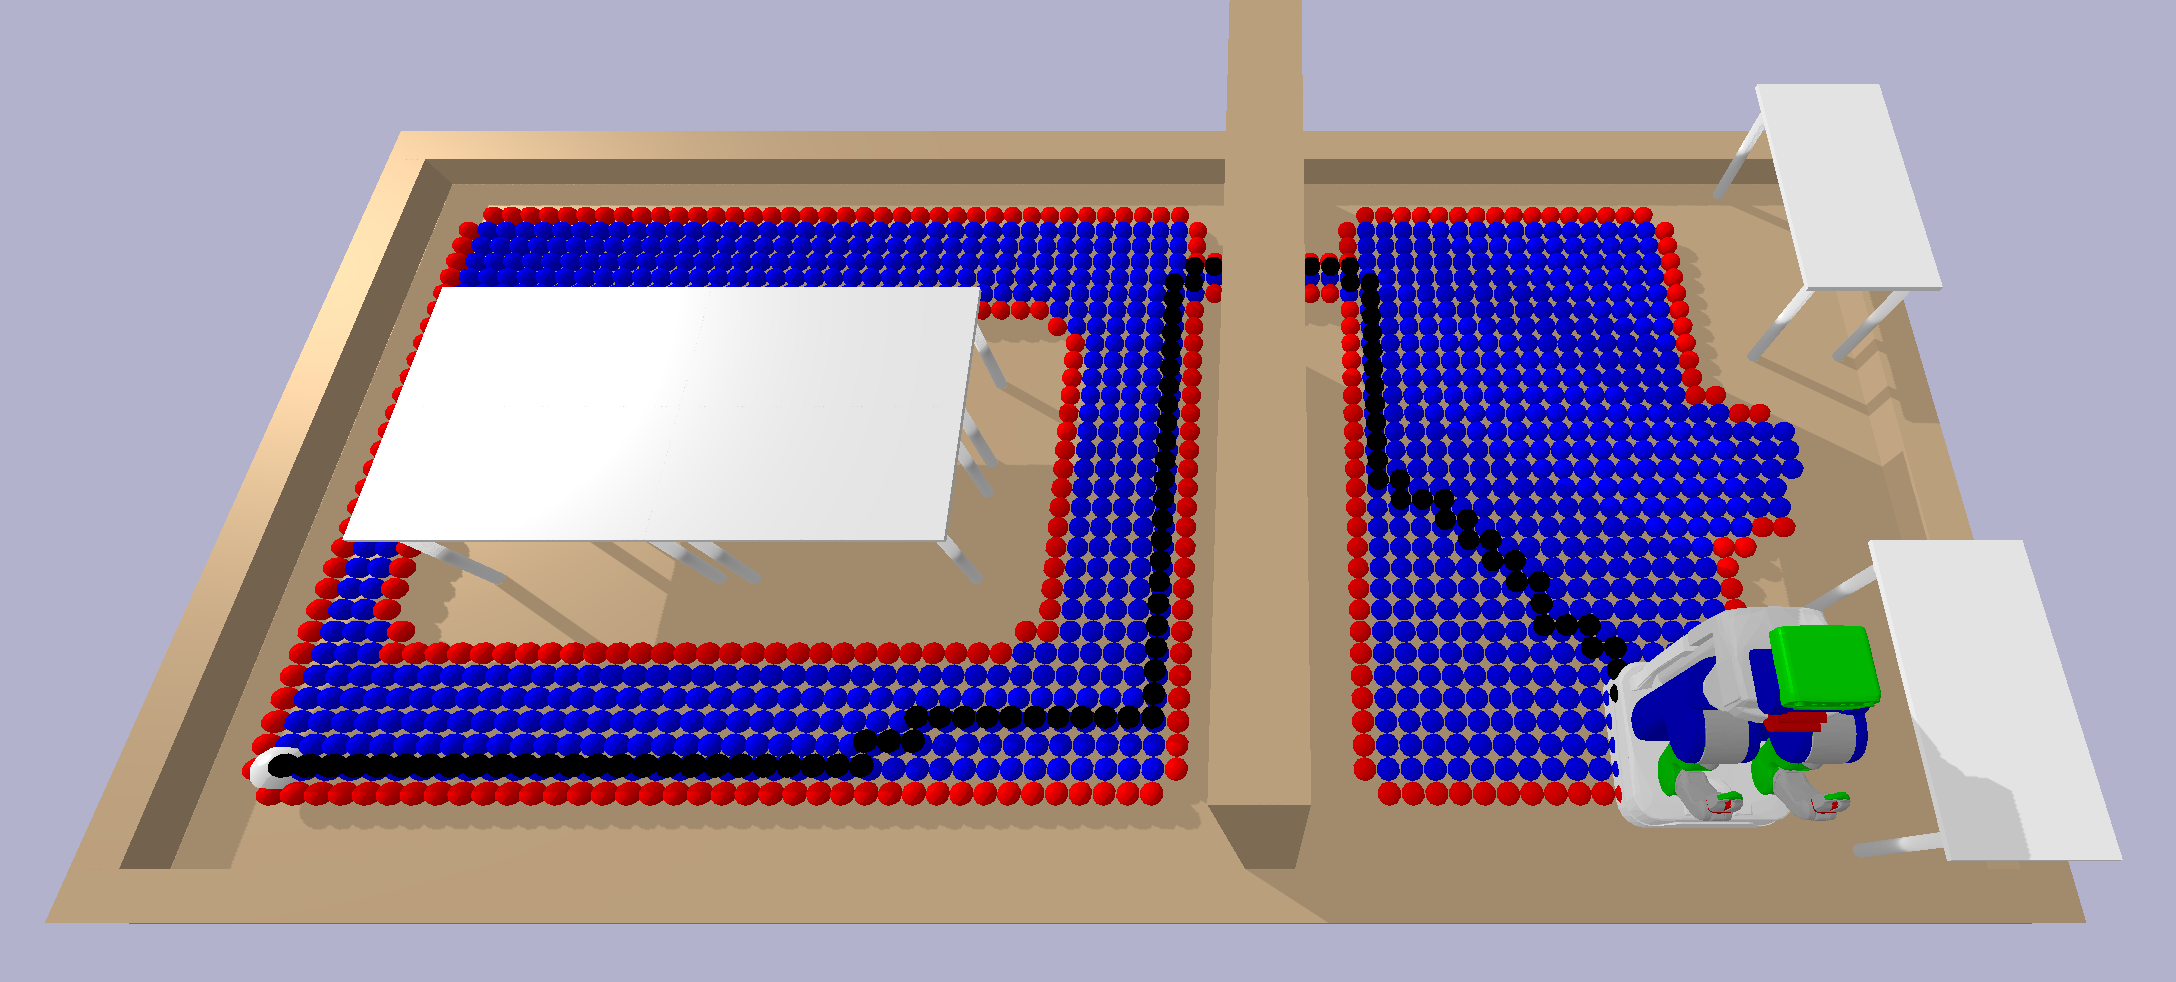
\includegraphics[width=0.8\columnwidth]{astar_4.png}}
        \caption{Visualization for explored configurations of 4-connected A* algorithm. The searched path is shown in black, the collision-free configurations are shown in blue and the colliding configurations are shown in red.}
        \label{fig:astar_4}
\end{figure}

\subsubsection*{b. 8-Connected variant}
% Astar finished with 7088 iterations
% OpenList length 7321, ClosedList length 4431
% Path Found!!!
% Path cost: 10.69553
% Planner run time:  7.526267766952515
Computation time: 7.5935 s

Path cost: 10.6955

\begin{figure}[H]
    \centering
        \textsf{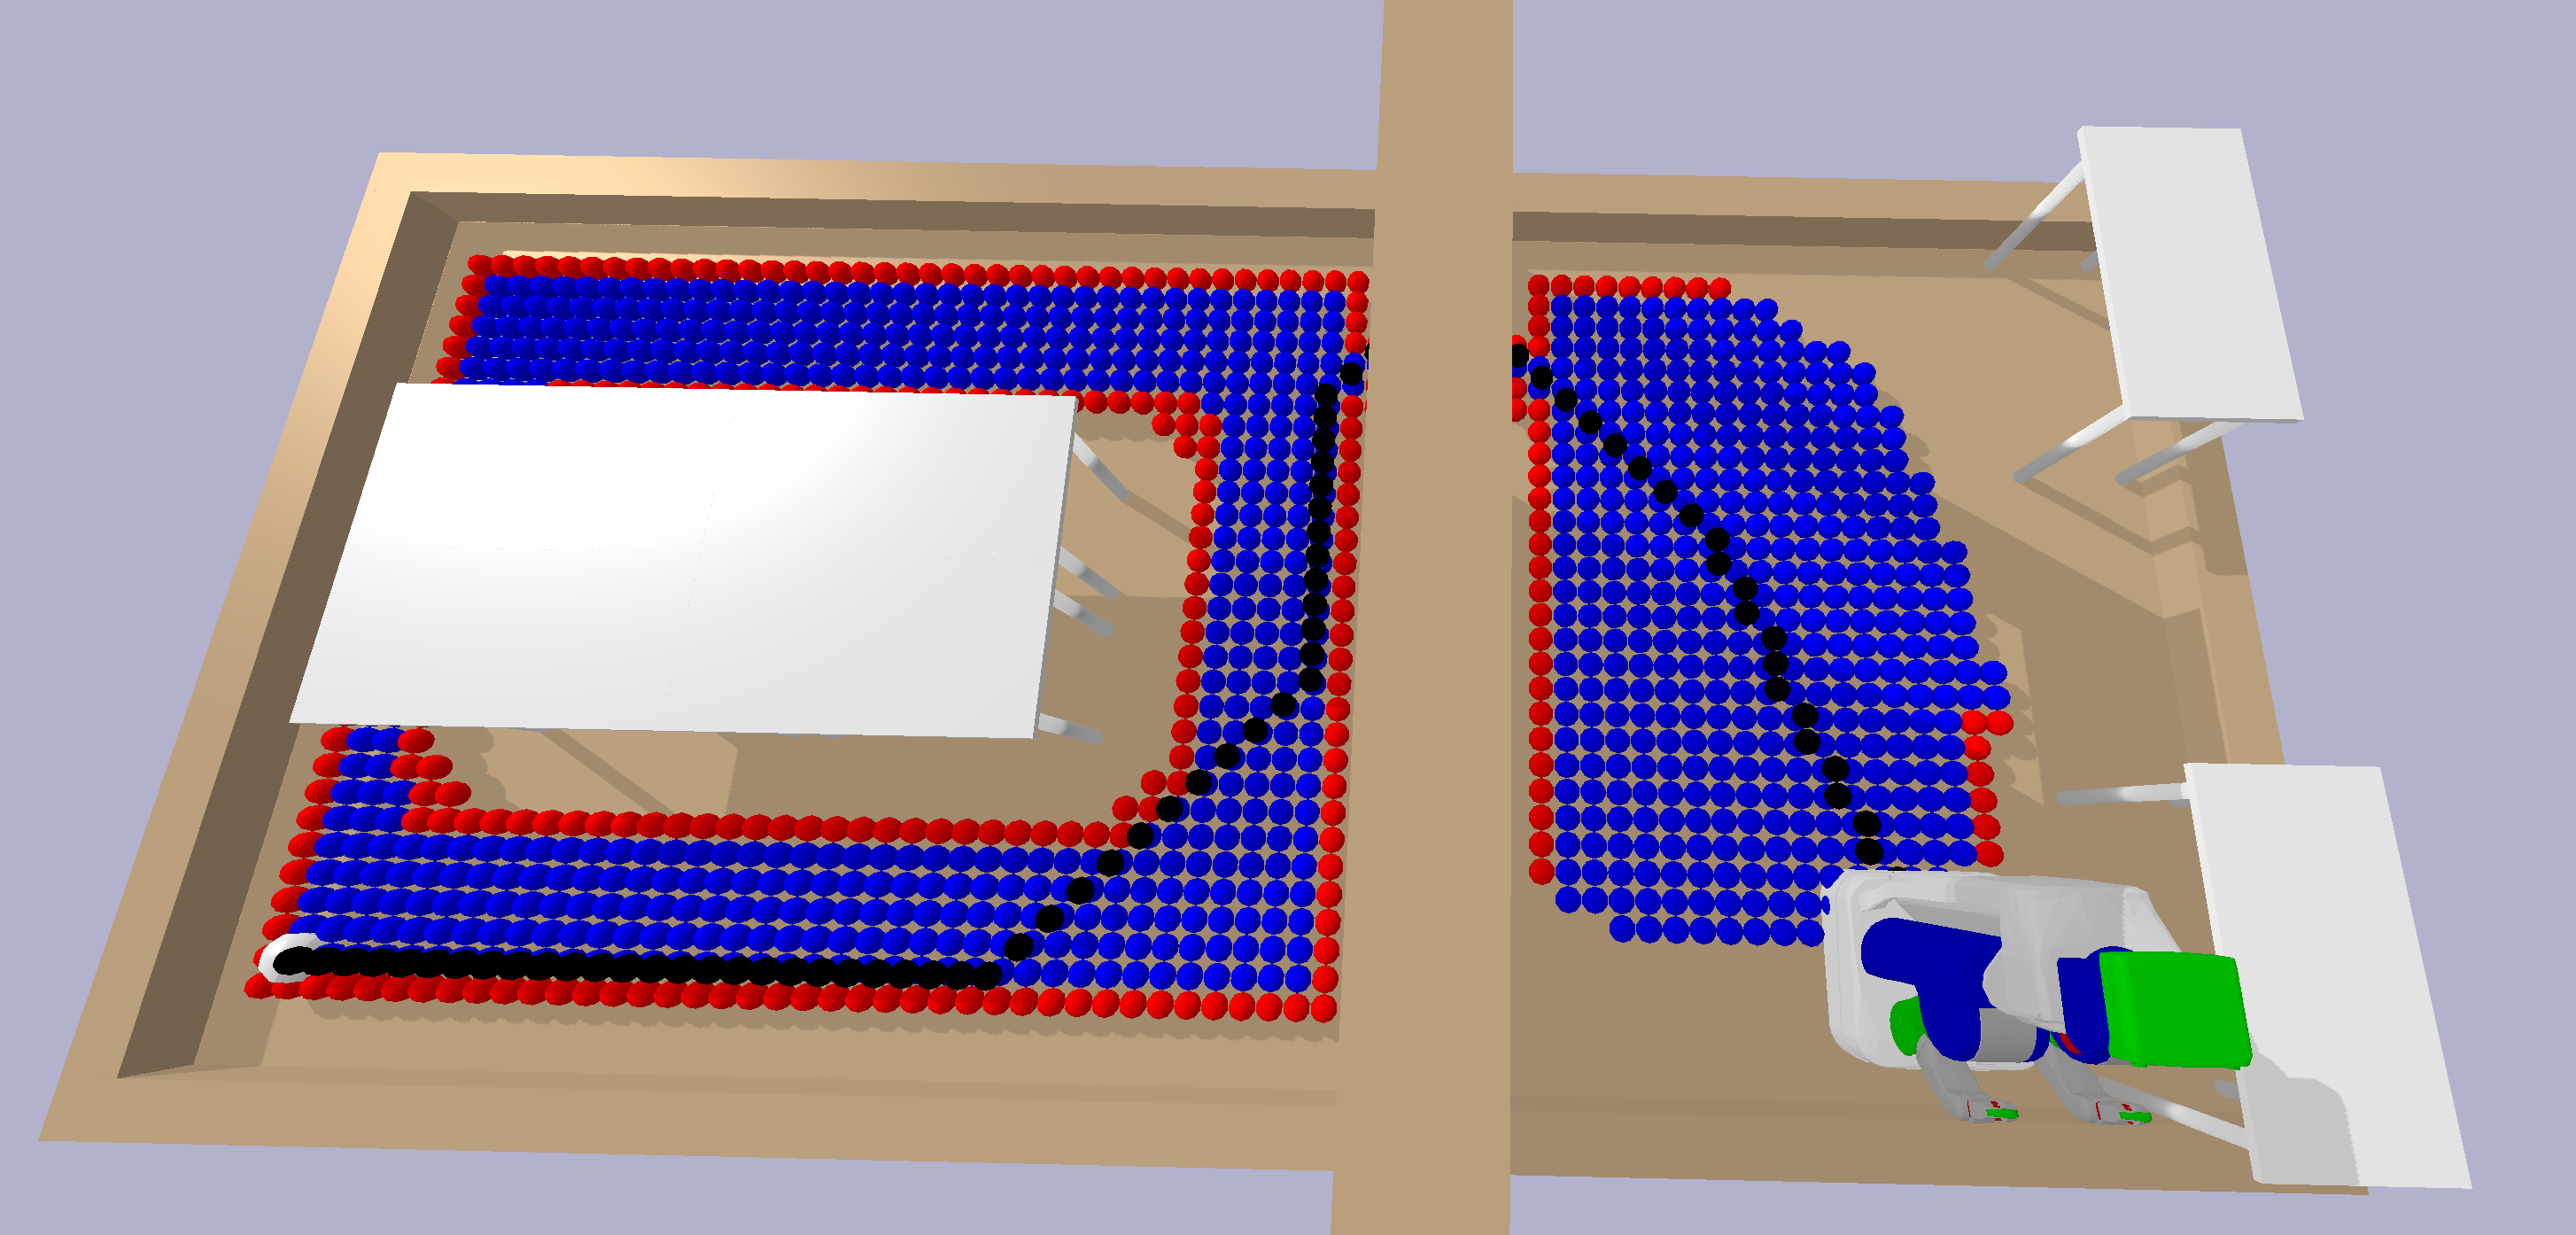
\includegraphics[width=0.8\columnwidth]{astar_8.png}}
        \caption{Visualization for explored configurations of 8-connected A* algorithm. The searched path is shown in black, the collision-free configurations are shown in blue and the colliding configurations are shown in red.}
        \label{fig:astar_8}
\end{figure}

\subsubsection*{c. Discussion}
% Which variant performs better in terms of computation time? Which variant performs better in terms of path cost? Explain why in the pdf.

\begin{table}[H]
	\centering
	\begin{tabular}{@{}lcc@{}}
		\toprule
		A* Variant           & 4-Connected & 8-Connected \\ 
		\midrule
		Computation Time (s) & 11.2534     & 7.5935  \\
		Path Cost            & 12.4708     & 10.6955 \\
		\# Expend Directions & 6           & 26      \\
		\# Iterations        & 9026        & 7088    \\
		Open List Length     & 3596    	   & 7321    \\ 
		Closed List Length    & 6628    	   & 4431    \\ 
		\bottomrule
	\end{tabular}
	\caption{Comparison of runtime statistic between two variants of A* algorithm. Run times are recorded on a laptop with i7-12700H CPU.}
	\label{tab:astar_cmp}
\end{table}

The 8-connected variant performs better in terms of both computation time and path cost as shown in Table \ref{tab:astar_cmp}.

It's obvious that the 8-connected variant need explore more nodes (11752) than the other (10224) since for each node it will explore more neighbor nodes around it, and it can utilize the diagonal direction of each config to find a path with lower accumulated action costs (10.6955) i.e. g cost than the other (12.4708) as well.

However, due to the fact that collision checking is far more computational expensive than other run time costs, the implementation can be optimized so that the variant with fewer iterations will run faster than the other.

It runs faster because fewer iterations are required and the most time expensive operation is processed only once in each iterations. There are two main sources for the run time expense, the first and dominant one is the collision checking process and the second one is the lookup of the closed list. They are necessary conditions to check for each explored nodes, but there are also two slots to choose for checking these conditions. One is right after getting the lowest cost node from the Open List and the other is when a neighbor node is explored. As long as both of them are checked once in total for both slots, the optimality of the searched path is reserved. Thus, to trade off the computation time over the number of explored nodes, check both collision and closed list at the first slot and check only closed list at the second slot will result in the fewer iterations while keep the number of explored nodes at a reasonable amounts (the more checks, the fewer nodes will be explored), so that makes the 8-connected variant faster.



\subsection*{Rapidly-Exploring Random Tree (RRT)}

\begin{figure}[H]
    \centering
        \textsf{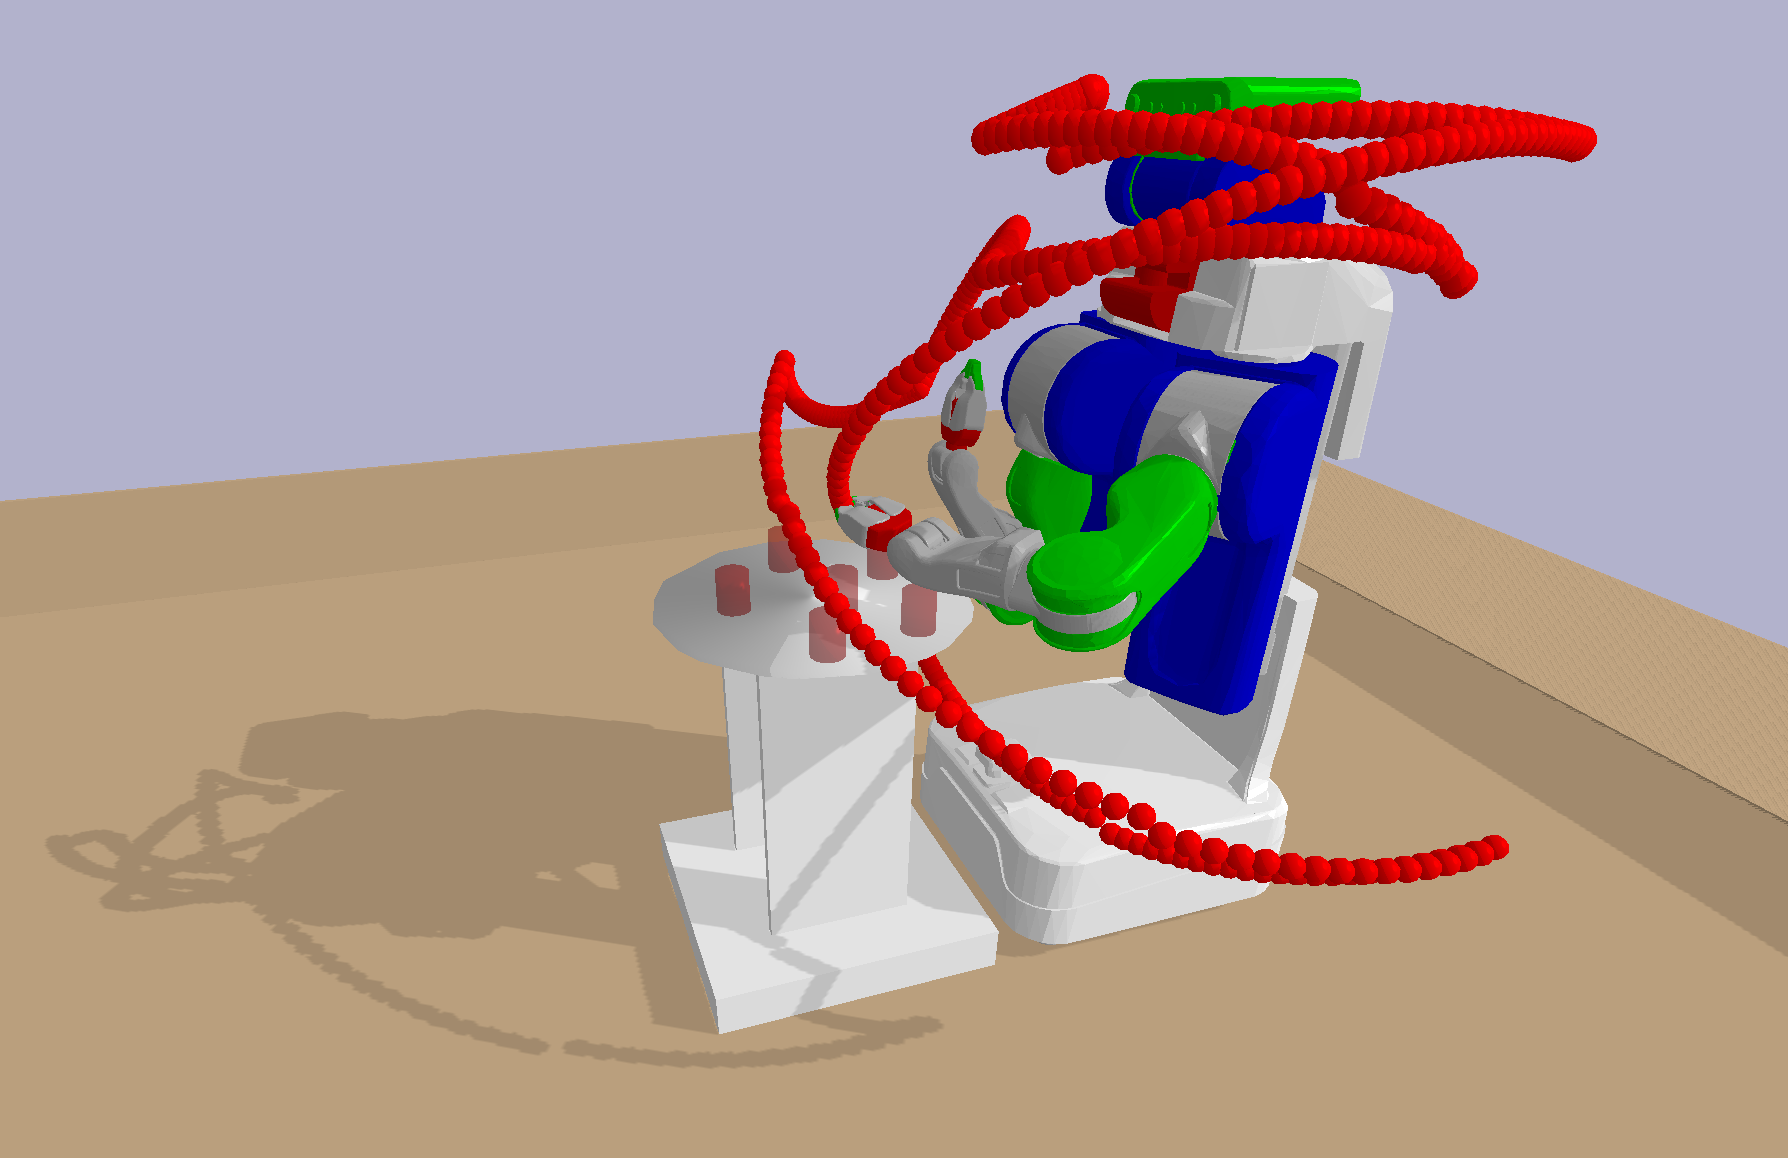
\includegraphics[width=0.7\columnwidth]{rrt_raw.png}}
        \caption{Visualization for searched path of the left end-effector in red.}
        \label{fig:rrt_raw}
\end{figure}

\begin{figure}[H]
    \centering
        \textsf{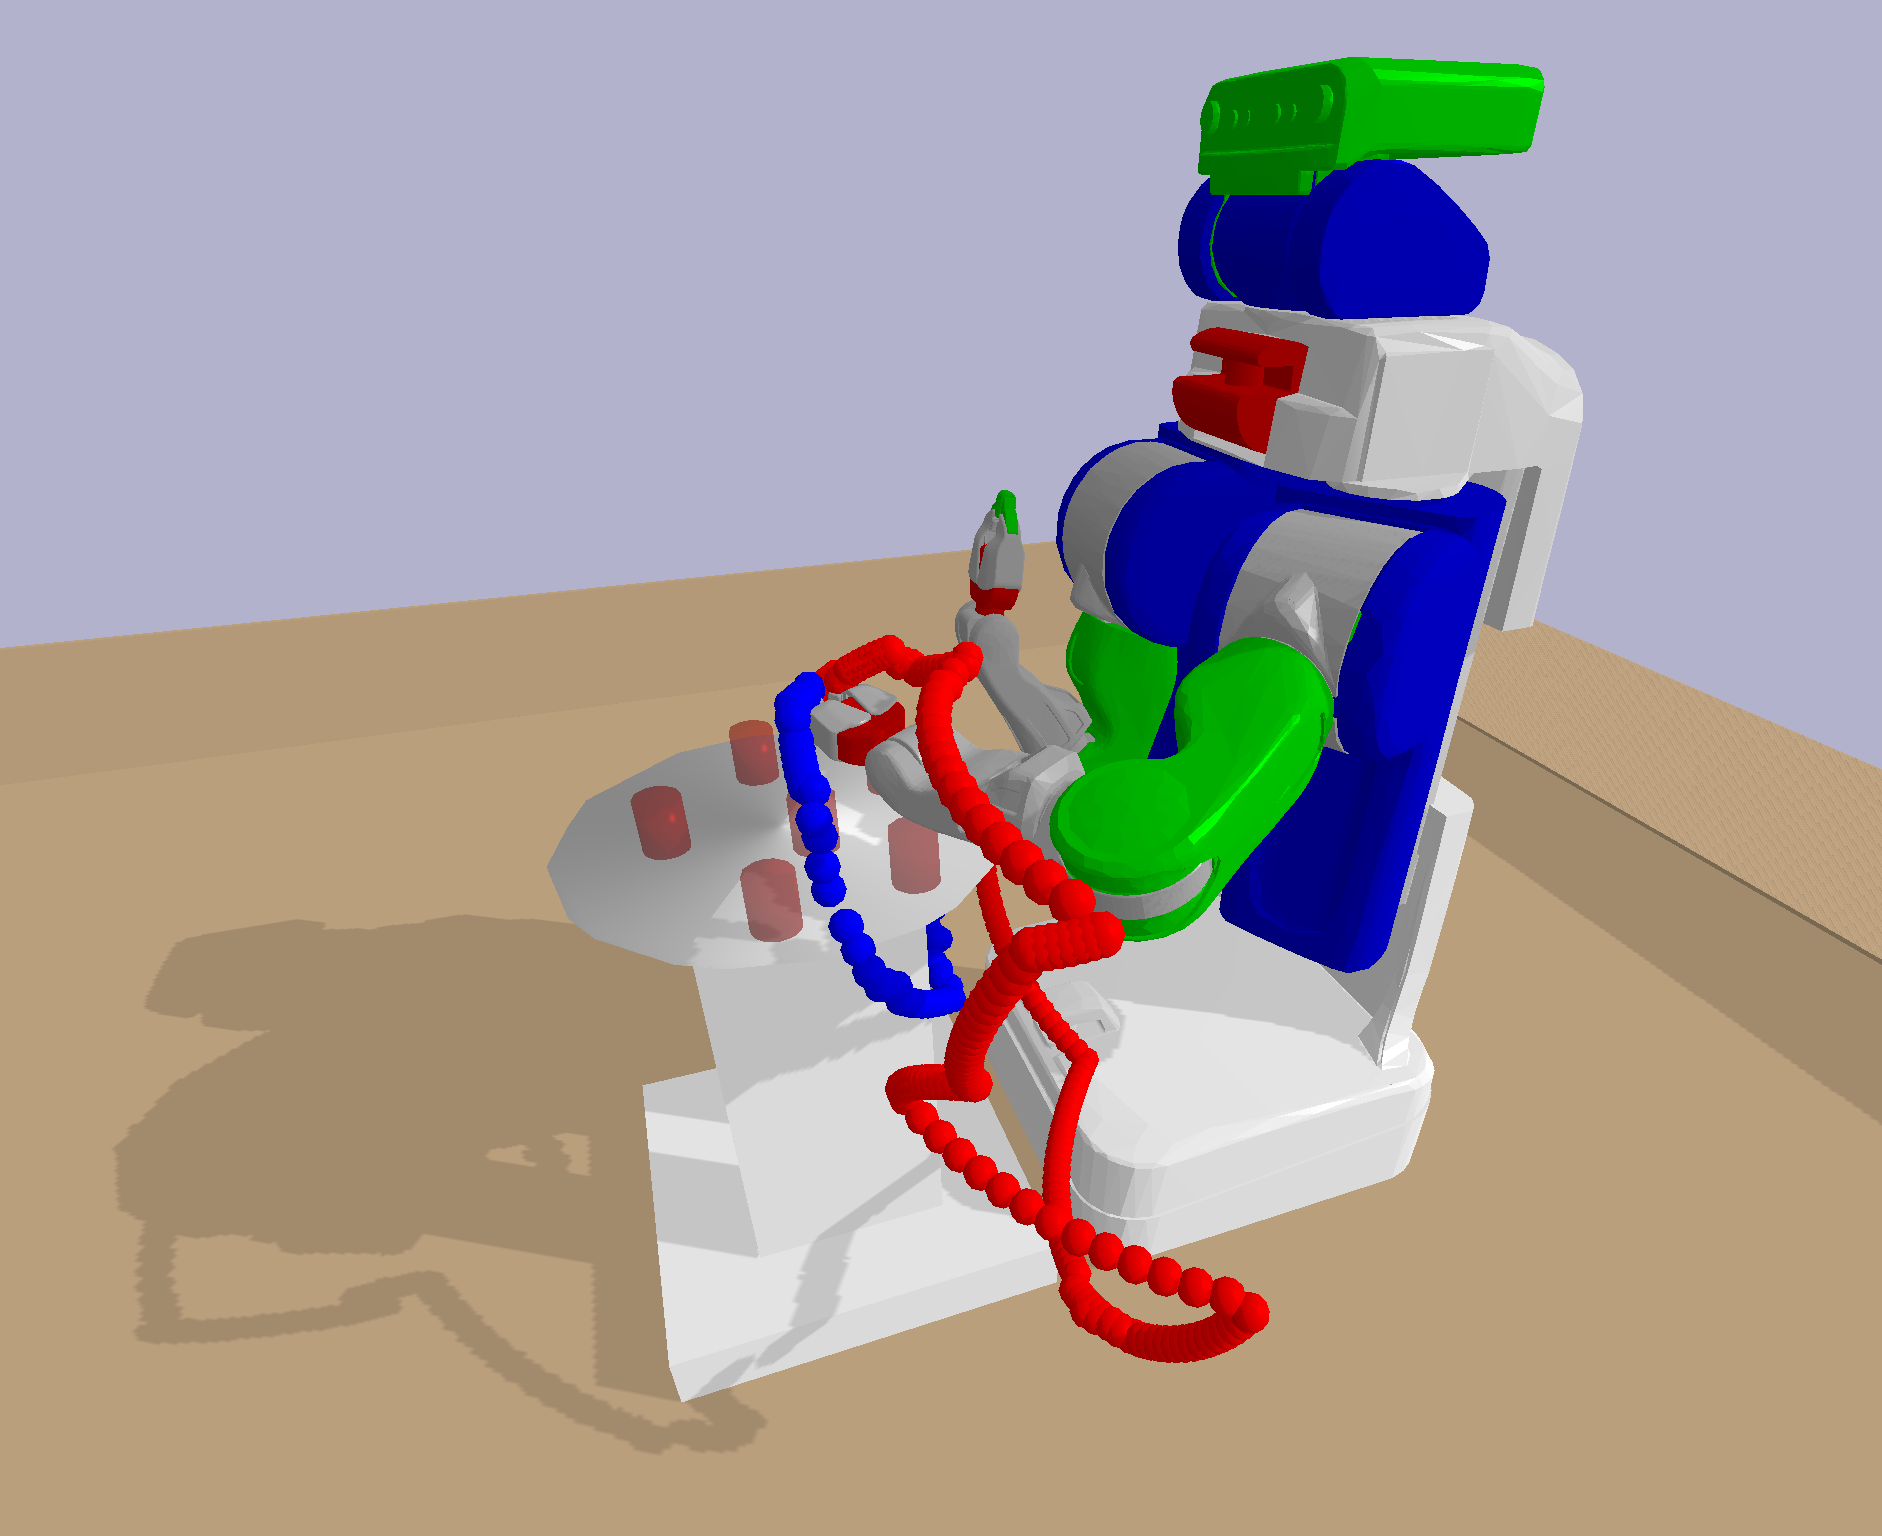
\includegraphics[width=0.7\columnwidth]{rrt_smoothed.png}}
        \caption{Visualization for searched path of the left end-effector in red and the shortcut-smoothed path in blue.}
        \label{fig:rrt_smoothed}
\end{figure}

\clearpage % this will flush any waiting float while \newpage won't
\appendix

\section{Fun Facts}
This appendix aims to discuss some fun facts and interesting characteristics of both A* and RRT algorithm I explored during implementation.

\subsection*{A*}
\subsubsection*{a. Search with heuristic cost only, but get a much faster suboptimal result?}

\begin{figure}[h]
    \centering
        \textsf{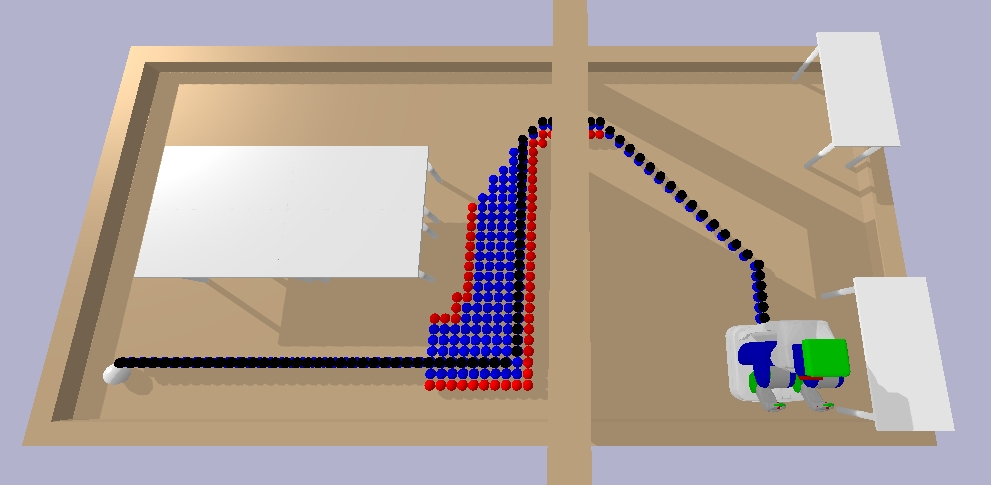
\includegraphics[width=0.8\columnwidth]{astar_no_gcost.png}}
        \caption{A* with heuristic cost only.}
        \label{fig:astar_no_gcost}
\end{figure}

This is only true if the $h(n)$ is very close the true cost and not an lower bound estimator (admissible), otherwise this is a disaster since the algorithm will just ignore the true cost of traveling from one node to the other (g cost) and result in a "imagined" optimal path. Indeed, the problem setup for this homework falls into the true case.

\subsubsection*{b. Enqueue any feasible neighbors and ignore nodes with lower g cost in open list, but get same result?}

This is true for problems I have solved so far. The mechanism behind is just let the priority queue to sift up the node with lower cost and let the closed list to handle those duplicated configs. The drawback of this is that much more unnecessary nodes are enqueued so typically requires more iterations and slows down the run time.


\subsection*{RRT}
\subsubsection*{a. Fun thing to try. Apply RRT to the first scenario?}

\begin{figure}[h]
    \centering
        \textsf{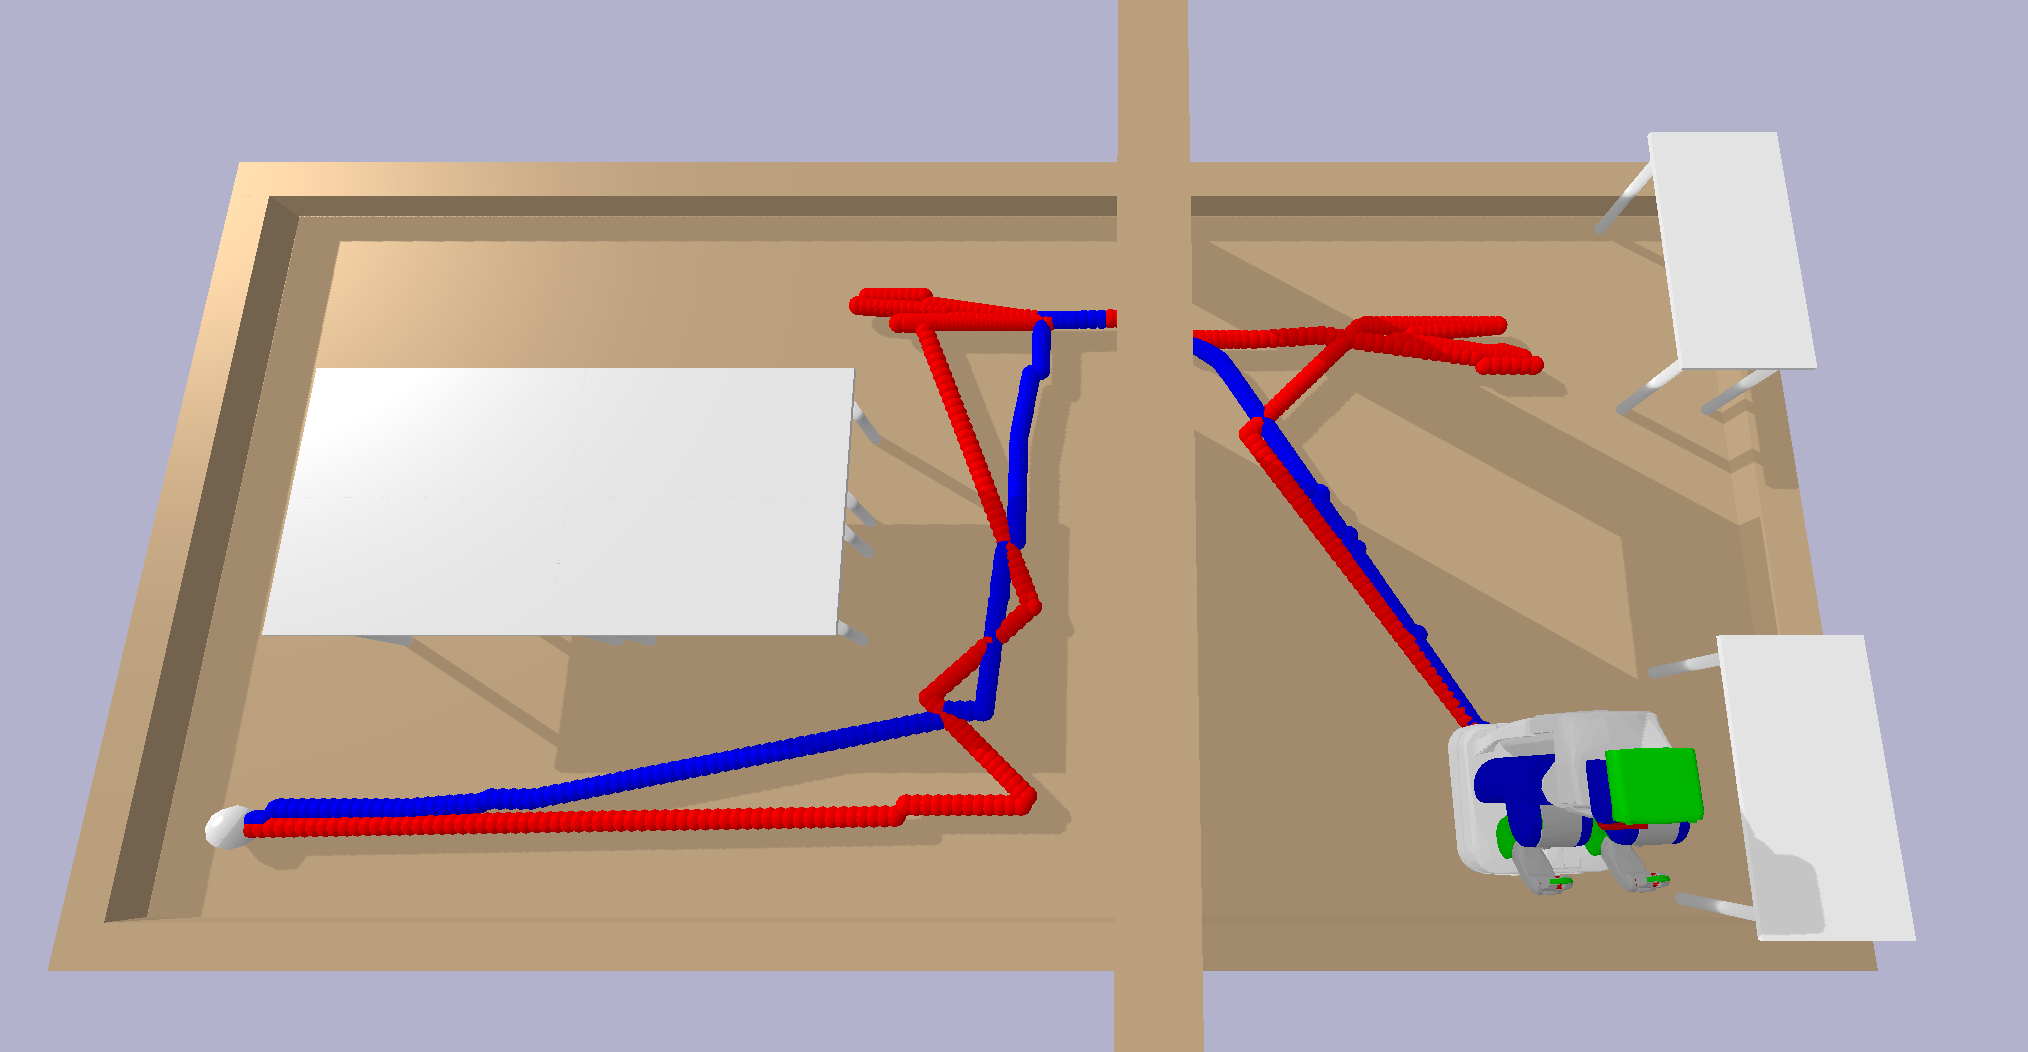
\includegraphics[width=0.8\columnwidth]{rrt_path.png}}
        \caption{Use RRT for path finding.}
        \label{fig:rrt_path}
\end{figure}

It works perfectly fine (Figure \ref{fig:rrt_path}), as expected, even though all config dimensions are treated as linear (no special distance wrap e.g. superior arc).

% \subsubsection*{b. How to boost nearest distance calculation speed?}

% Since the convergence time for a single tree RRT is usually a bit random, and the most expensive steps for it is to find the nearest node, find a way to boost the calculation speed and keep it almost independent to the number of nodes could help save convergence time a lot.

% There is a few ways to find the nearest node between the RRT tree and the target node, and a few underlining containers can be used to store the tree.
% The most used data structure to find the nearest neighbor in high dimensions is the KD-Tree, but it is too expensive to add new nodes in each iteration for this problem.
% TODO how to add KDTree in RRT? combine a list and a tree!
% TODO build a list first and once its length reach e.g. 2000, build a KDTree, then query the tree for NN and keep building the list, query the true NN by combining the result from KDTree and the list, build a tree again once the length of the list reach e.g. 2000 again.
% Therefore, the remaining choices are python list, numpy ndarray and a mixed version (use list to append and convert to ndarray to calculate distance).

% The key idea is to avoid any for loop and calculate the distance in the vectorized form (i.e. matrix), so I compared the three choices and found that using the last two can already boost about 10 times faster then using only python list when the number of nodes are fewer than 5000.


\end{document}